\section{Introduction}\label{introduction}

\begin{frame}{Women Contribute Online Less Than Men}

\begin{itemize}[<+->]
\tightlist
\item
  Only 13\% women contributors on Wikipedia
\item
  Wikipedia entries about women are less likely to be complete
\item
  Only 5\% women contributors on StackOverflow
\item
  Less than 5\% women taking part in programming competitions (despite
  30\% in CS schools)
\end{itemize}

\end{frame}

\begin{frame}{Implications for individuals, firms \& society}

\textbf{Profits} of online companies (e.g., Airbnb)

\begin{itemize}
\tightlist
\item
  Narrow participation \(\leadsto\) lower profits
\item
  Less diversity \& creativity for innovation
\end{itemize}

\pause

\textbf{Labor market discrimination}

\begin{itemize}
\tightlist
\item
  Signaling skills
\item
  Learning
\end{itemize}

\pause

\textbf{Cultural} discrimination

\begin{itemize}
\tightlist
\item
  Platform content may reflect biased views
\end{itemize}

\end{frame}

\begin{frame}{A theory of gender imbalance}

Many factors to consider (see Lam et. al 2011)

We conjecture:

\begin{itemize}
\tightlist
\item
  \textbf{Gamification} \& Incentives (e.g., competition, points,
  rankings)
\item
  Gender differences in \textbf{preferences} (e.g., risk aversion,
  competitive inclination)
\end{itemize}

\pause

\textbf{Mechanisms} under investigation

\begin{enumerate}
\def\labelenumi{\arabic{enumi}.}
\tightlist
\item
  Perceived gender composition in a competitive environment.
\item
  \color{gray}{Collaboration incentives under gender imbalance [next study]}
\end{enumerate}

\end{frame}

\section{The role of the perceived gender
imbalance}\label{the-role-of-the-perceived-gender-imbalance}

\begin{frame}{Bayesian updating}

\begin{figure}
\centering
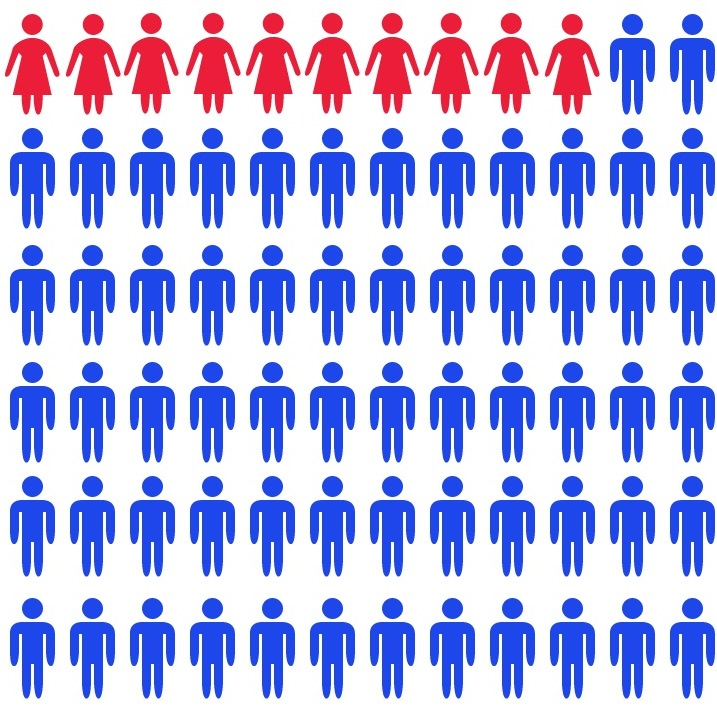
\includegraphics{female_fuel_for_the_digital_economy.jpg}
\caption{What are the odds of winning for gender XY?}
\end{figure}

\end{frame}

\begin{frame}{Role model}

\begin{figure}
\centering
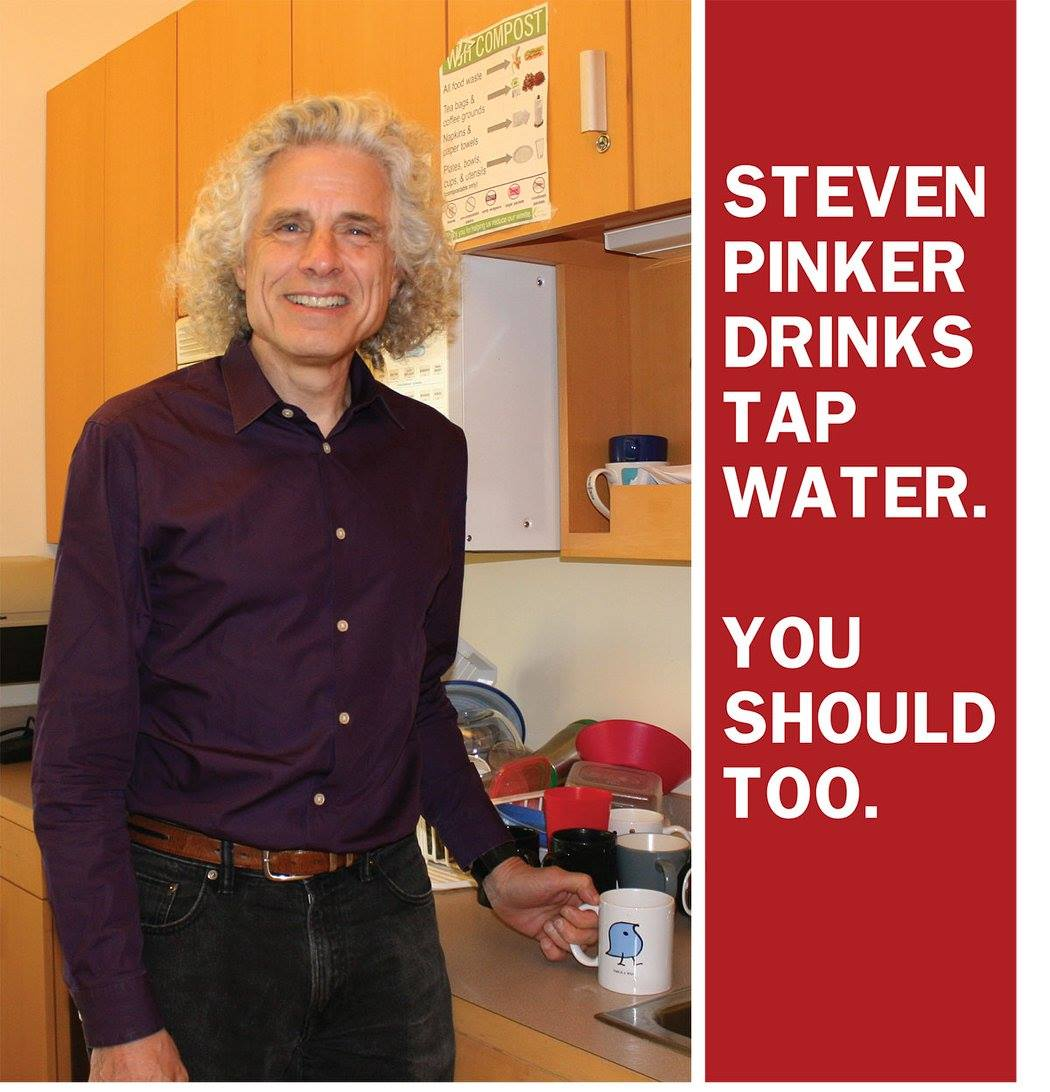
\includegraphics[width=0.5\textwidth]{tap_water_pinker.jpg}
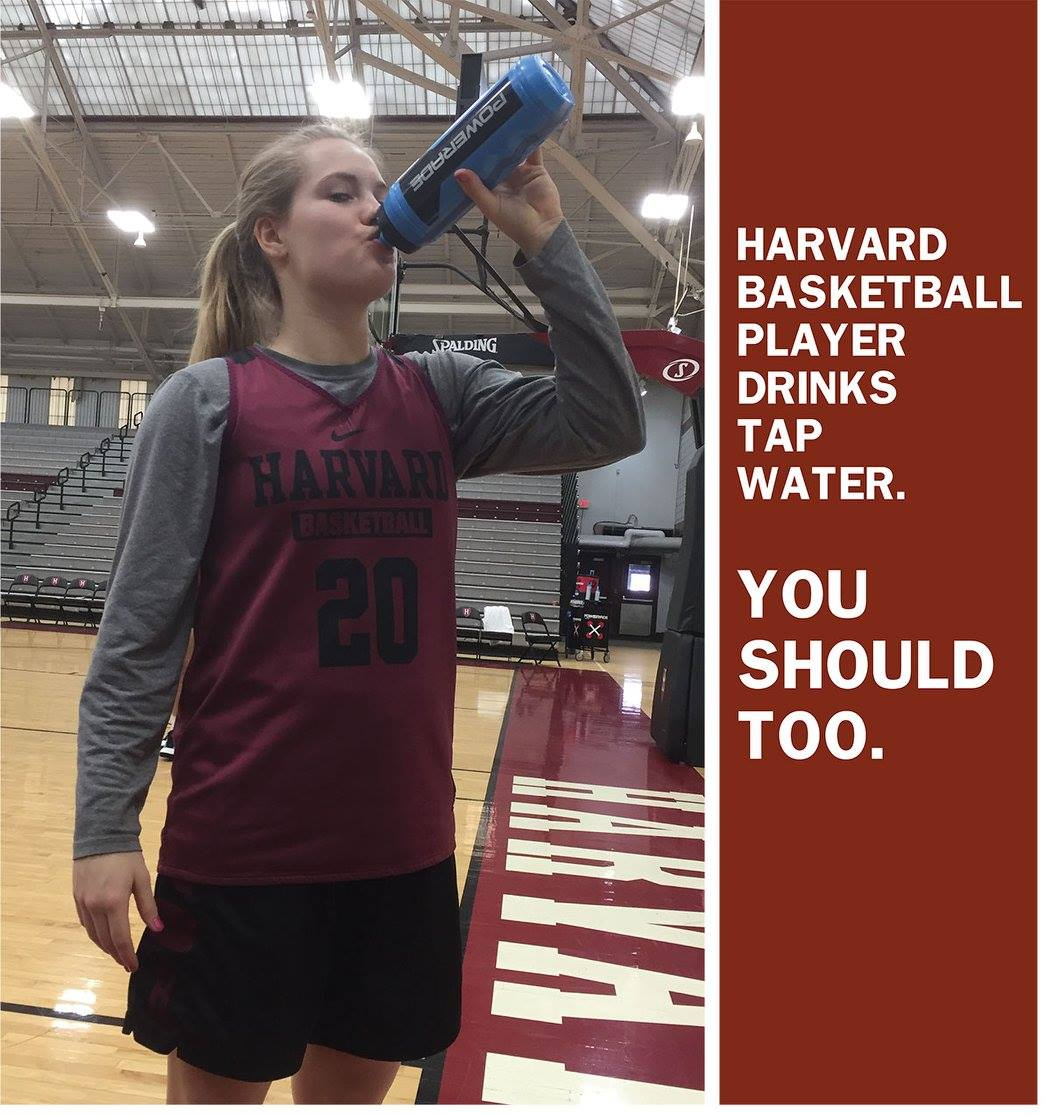
\includegraphics[width=0.5\textwidth]{tap_water_basket.jpg}
\caption{do I want to be successful in this?}
\end{figure}

\end{frame}

\begin{frame}

\begin{figure}
\centering
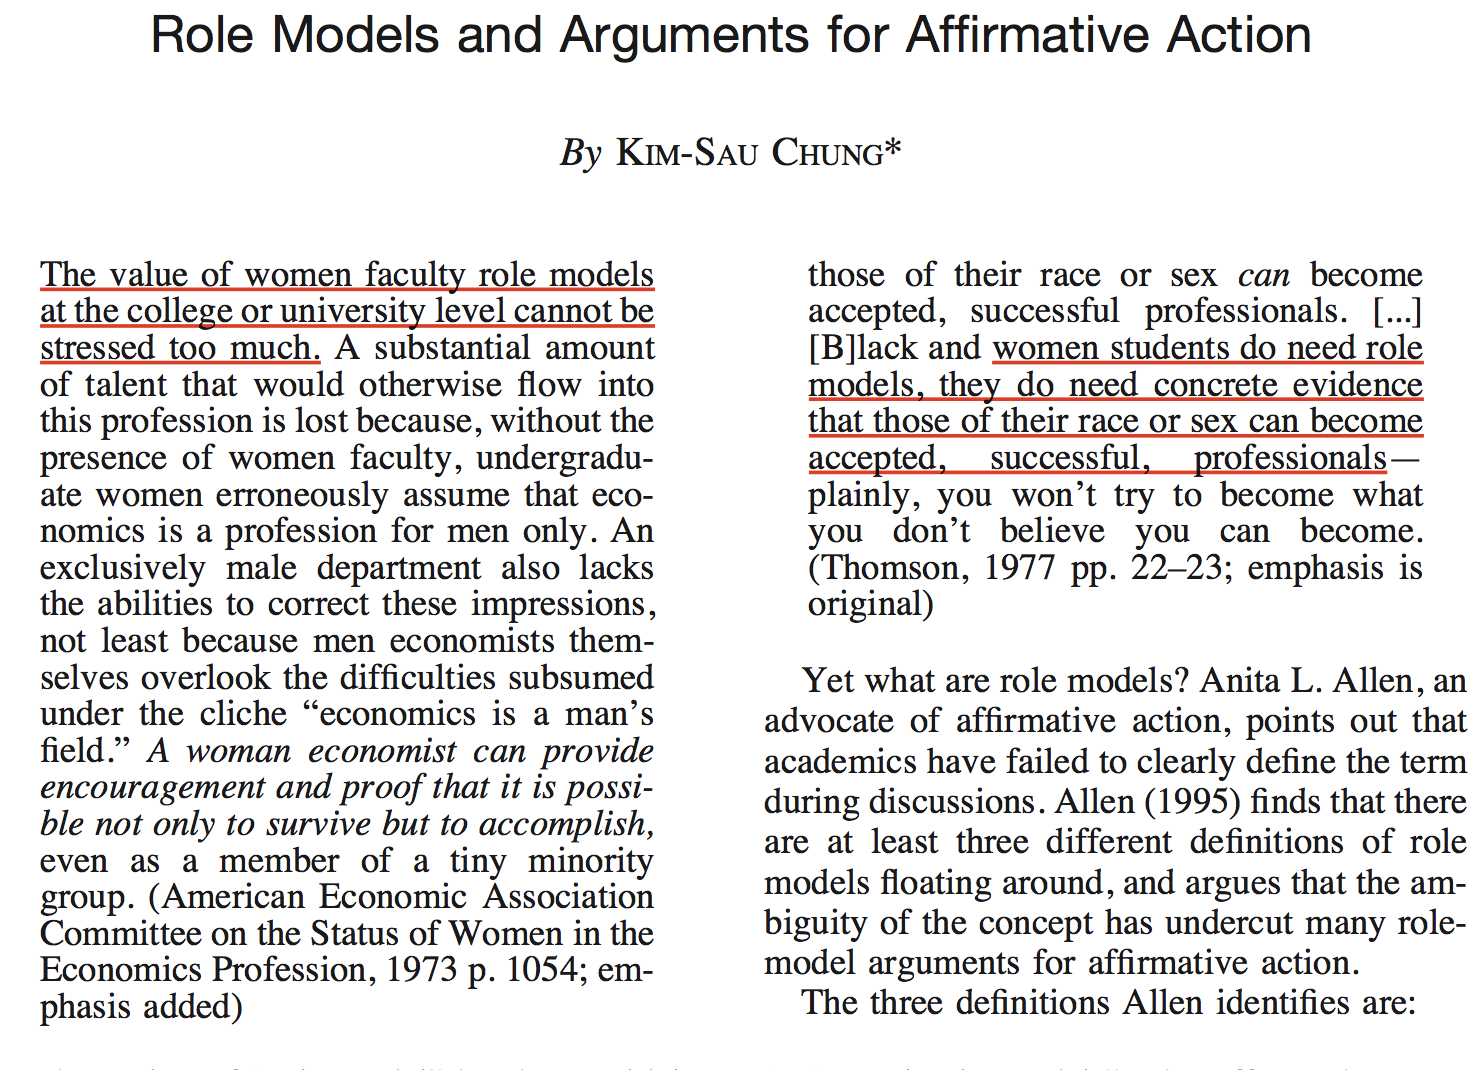
\includegraphics{aer-citation.png}
\caption{American Economic Review, 2000}
\end{figure}

\end{frame}

\section{Context and Data}\label{context-and-data}

\begin{frame}{Herox.com}

The sex ratio is:

\begin{itemize}
\tightlist
\item
  2 men registrants for each woman (33 percent women)
\item
  3 men contributing for each woman (25 percent women)
\end{itemize}

\end{frame}

\begin{frame}

\begin{figure}
\centering
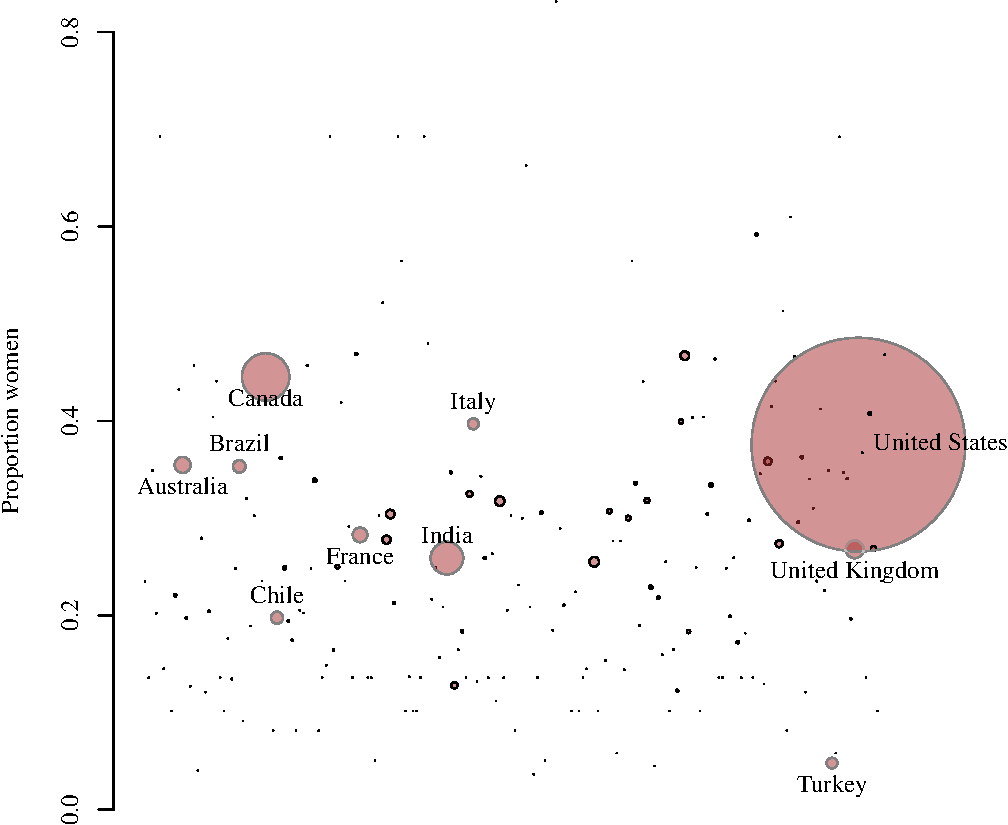
\includegraphics{report_slides_files/figure-beamer/bayes-1.pdf}
\caption{Proportion of women members by country}
\end{figure}

\end{frame}

\begin{frame}

\begin{figure}
\centering
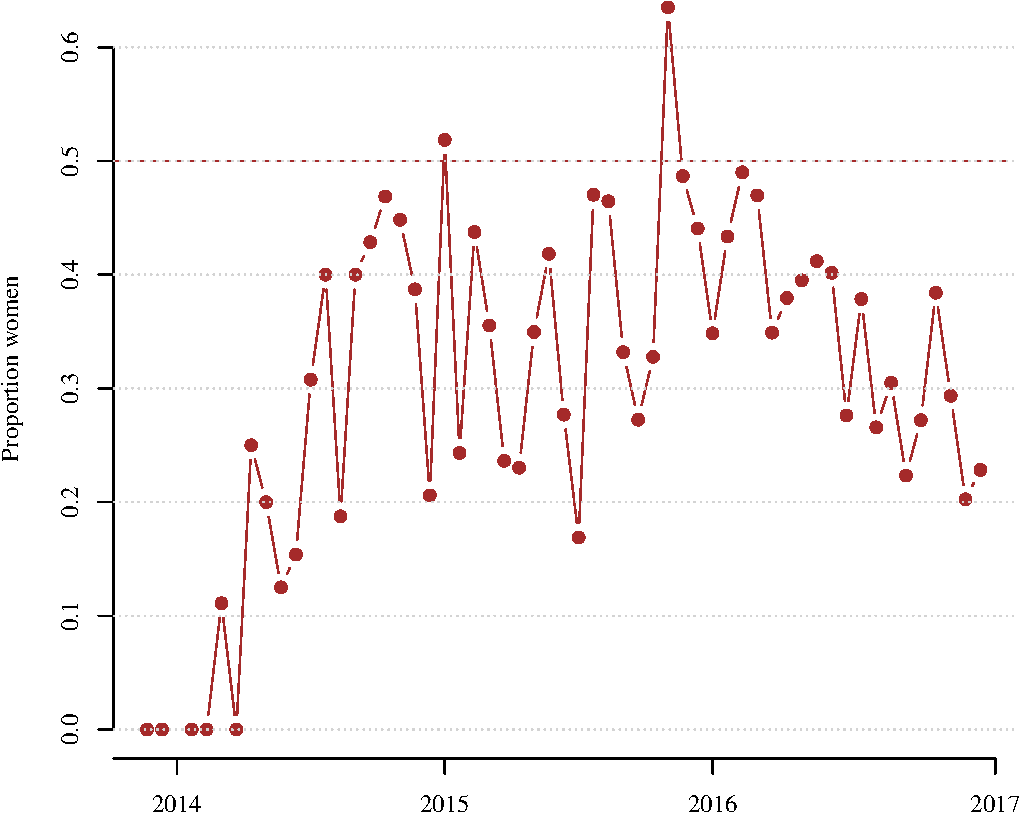
\includegraphics{report_slides_files/figure-beamer/overtime-1.pdf}
\caption{Proportion of women new members over time}
\end{figure}

\end{frame}

\begin{frame}

\begin{figure}
\centering
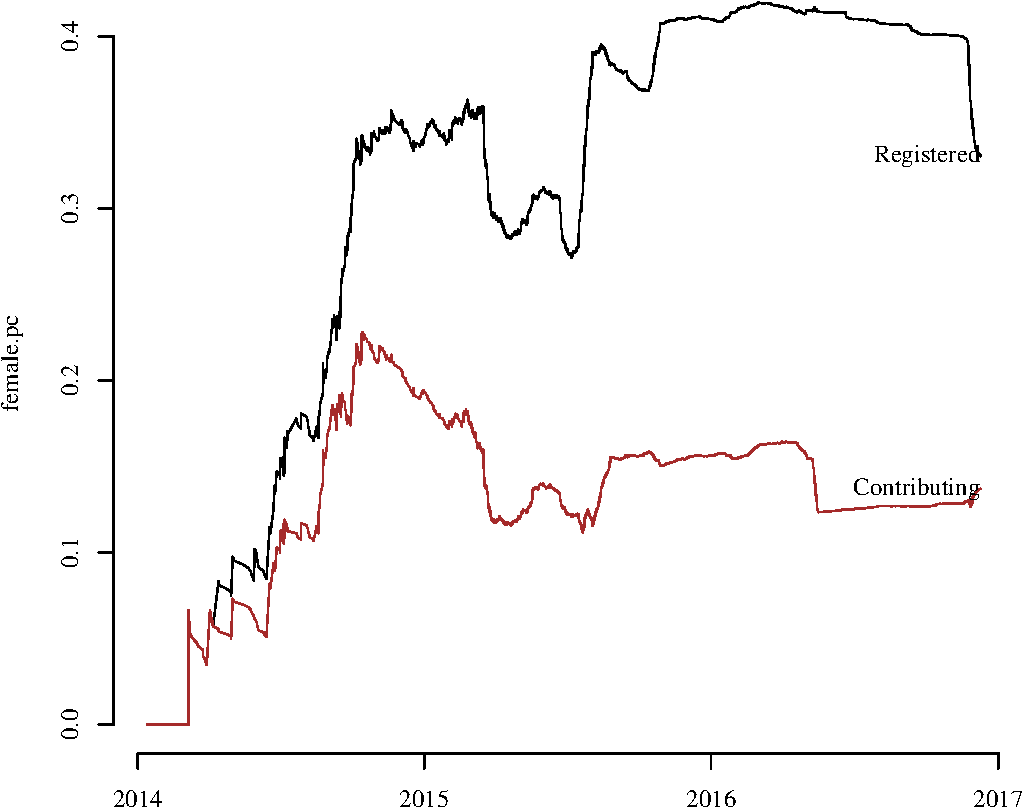
\includegraphics{report_slides_files/figure-beamer/cumsum-1.pdf}
\caption{Cumulative proportion of women over time}
\end{figure}

\end{frame}

\section{Experimental design}\label{experimental-design}

\begin{frame}{How to influence the perceived gender composition?}

Featuring 2-3 member profiles.

\begin{itemize}
\item
  experience + bio + profile picture
\item
  ADD regression controls for past experience on platform
\end{itemize}

\end{frame}

\begin{frame}{Example of HeroX's member}

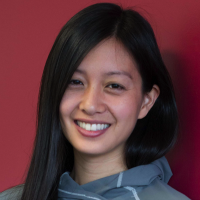
\includegraphics[width=1.0in]{jessica.png}

\begin{quote}
Jessica is currently wrapping up as a graduate student at Stanford. She
led youth engagement at D-Lab at the Massachusetts Institute of
Technology, which collaborates with communities facing economic poverty
to design technologies to improve quality of life. She co-founded a
social enterprise based in West Bengal, India that aims to increase
access to clean drinking water through affordable community chlorination
devices.
\end{quote}

\end{frame}

\begin{frame}{Whom to influence?}

Registered members (increase participation)

\begin{itemize}
\tightlist
\item
  Direct solicitation email
\end{itemize}

Not yet registered members (foster registration \& participation)

\begin{itemize}
\tightlist
\item
  Mailing lists, Facebook ads, etc. (can we track?)
\end{itemize}

\end{frame}

\begin{frame}{Example email solicitation}

\begin{figure}
\centering
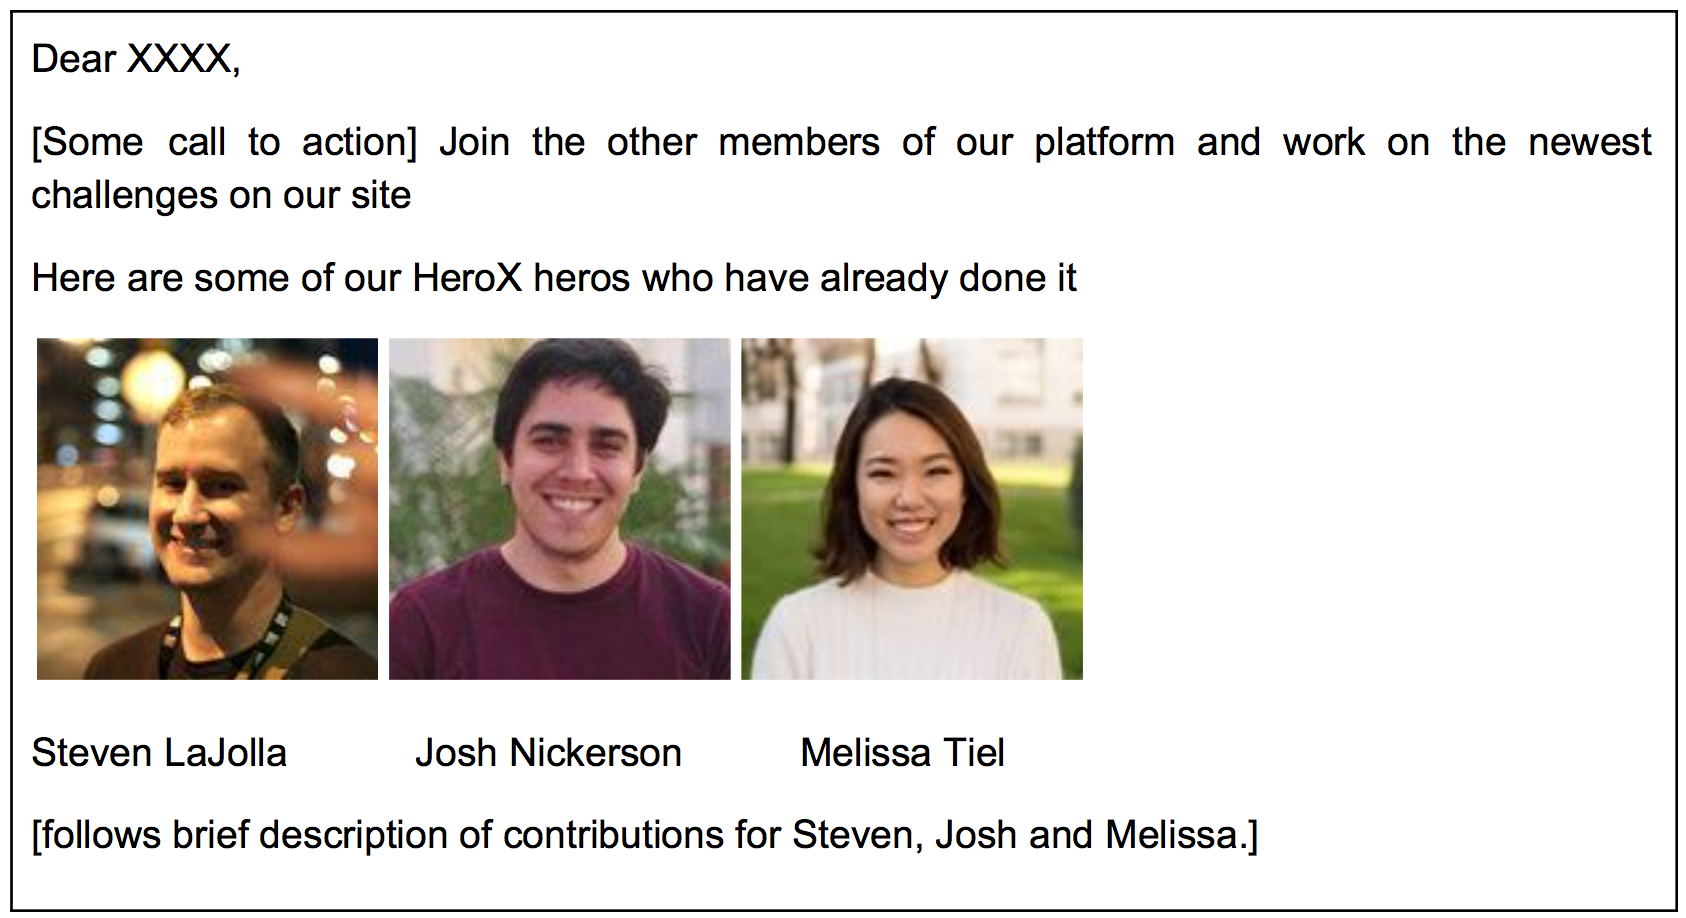
\includegraphics{solicit_gender_compo.png}
\caption{Solicitation email}
\end{figure}

\end{frame}

\begin{frame}{Treatment}

\begin{itemize}
\tightlist
\item
  Vary gender composition (look at ``Tokenism'')
\item
  Vary ``success'' composition
\end{itemize}

\begin{table}[ht]
\centering
\begin{tabular}{rll}
  \hline
 & Var1 & Var2 \\ 
  \hline
1 & 1 man role model & 3 women \\ 
  2 & 1 woman role model & 3 women \\ 
  3 & 1 man role model & 1 man 2 women \\ 
  4 & 1 woman role model & 1 man 2 women \\ 
  5 & 1 man role model & 2 men 1 woman \\ 
  6 & 1 woman role model & 2 men 1 woman \\ 
  7 & 1 man role model & 3 men \\ 
  8 & 1 woman role model & 3 men \\ 
   \hline
\end{tabular}
\caption{Treatment combinations} 
\end{table}

\end{frame}

\begin{frame}{Facebook/Twitter ads}

\begin{figure}
\centering
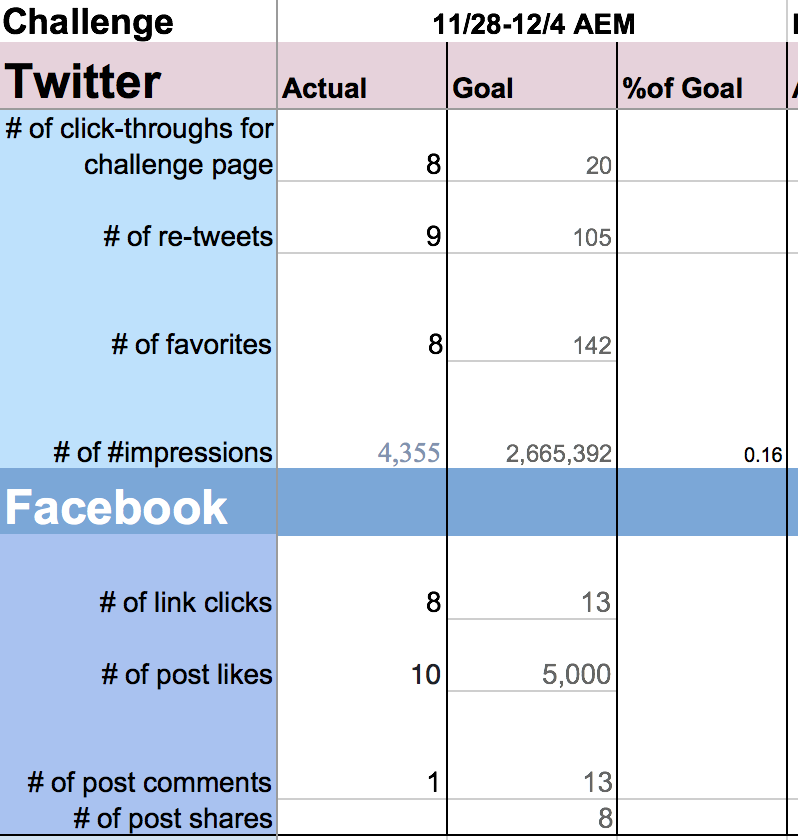
\includegraphics{ads.png}
\caption{Some statistics}
\end{figure}

\end{frame}

\begin{frame}{Validation of profiles}

Goal: comparable profiles

Use demographics + in the lab ratings of 20-30 profiles

\begin{itemize}
\tightlist
\item
  Physical attractiveness (based on user profile picture)
\item
  Role model (bio description + picture)
\item
  Skills
\end{itemize}

\end{frame}

\begin{frame}{Timing of the experiment}

\begin{enumerate}
\def\labelenumi{\arabic{enumi}.}
\tightlist
\item
  Preliminary survey (calibrate perceived gender composition)
\item
  Solicitation (email sent 1-2 times)
\item
  Ex-post survey (detect possible changes on perceived gender
  composition)
\end{enumerate}

\begin{itemize}
\tightlist
\item
  Outcome variables: participation, effort, team formation, etc.
\end{itemize}

\end{frame}

\begin{frame}{Example survey}

\begin{enumerate}
\def\labelenumi{\arabic{enumi}.}
\tightlist
\item
  Demographics (age, gender)
\item
  Motivations to participate in HeroX

  \begin{itemize}
  \tightlist
  \item
    {[}Cash prizes{]}
  \item
    {[}Learning{]}
  \item
    {[}CV/job opportunity{]}
  \item
    {[}Help society{]}
  \end{itemize}
\item
  What challenges do you like?

  \begin{itemize}
  \tightlist
  \item
    {[}STEM{]}
  \item
    {[}Social impact{]}
  \item
    {[}else{]}
  \end{itemize}
\item
  Estimate platform composition?

  \begin{itemize}
  \tightlist
  \item
    {[}Gender{]}
  \item
    {[}Age{]}
  \end{itemize}
\end{enumerate}

\end{frame}

\begin{frame}{Next steps}

\begin{enumerate}
\def\labelenumi{\arabic{enumi}.}
\tightlist
\item
  Identify profiles and ask for their consent (picture)
\item
  Recruit students to validate profiles
\item
  Send out preliminary survey
\item
  Ultimate solicitation message
\item
  Ads campaign with profiles
\item
  Examine results
\end{enumerate}

\end{frame}

\section{Collaboration incentives}\label{collaboration-incentives}

\begin{frame}{Basic idea}

\begin{enumerate}
\def\labelenumi{\arabic{enumi}.}
\tightlist
\item
  Male-female rich environment (how many teams?)
\item
  Splitting the pie rules (how many teams?)
\item
  Self-confidence
\end{enumerate}

\end{frame}

\begin{frame}{Technical requirements}

\begin{itemize}
\tightlist
\item
  Creating non-overlapping lists of potential teammates
\item
  Randomize composition of pool of potential teammates
\item
  Offer different incentives
\end{itemize}

\end{frame}

\begin{frame}{Example teaming}

\begin{figure}
\centering
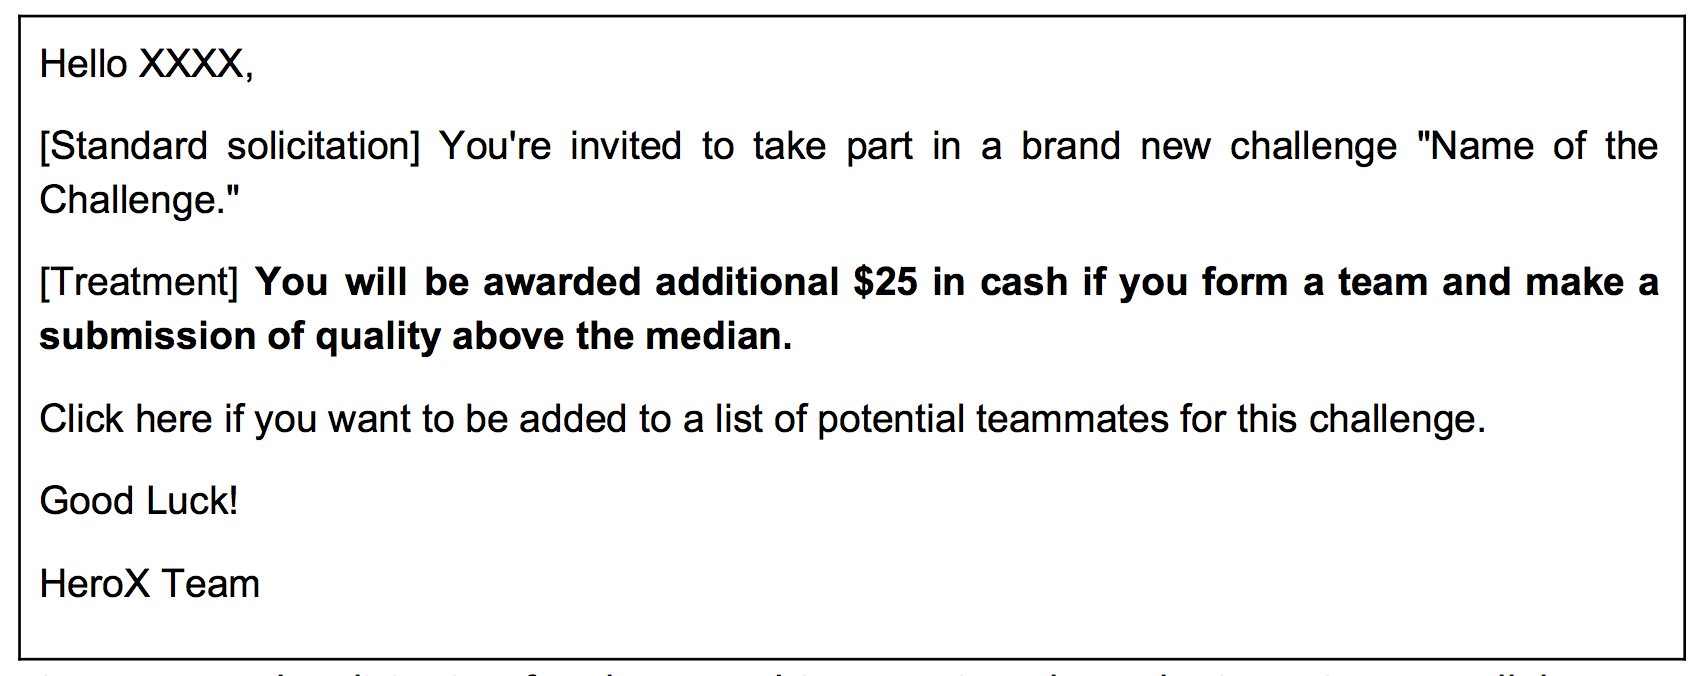
\includegraphics{solicit_teaming.png}
\caption{Teaming experiment}
\end{figure}

\end{frame}

\section{Thanks}\label{thanks}

\section{Demand estimation of the
challenges}\label{demand-estimation-of-the-challenges}

\begin{frame}[fragile]{Basic idea}

Launch \texttt{LinkedIn} campaign offering different pricing schemes

Examples:

\begin{enumerate}
\def\labelenumi{\arabic{enumi}.}
\tightlist
\item
  Fees vs no fees
\item
  Subsidizing prize money
\item
  Information treatment
\end{enumerate}

\end{frame}
